% Adjust these for the path of the theme and its graphics, relative to this file
%\usepackage{beamerthemeFalmouthGamesAcademy}
\usepackage{../../beamerthemeFalmouthGamesAcademy}
\usepackage{multimedia}
\graphicspath{ {../../} }

% Default language for code listings
\lstset{language=Python
}

% For strikethrough effect
\usepackage[normalem]{ulem}
\usepackage{wasysym}

\usepackage{pdfpages}

% http://www.texample.net/tikz/examples/state-machine/
\usetikzlibrary{arrows,automata}
\usetikzlibrary{tikzmark,calc}

\newcommand{\modulecode}{COMP260}\newcommand{\moduletitle}{Distributed Systems}\newcommand{\sessionnumber}{5}

\begin{document}
\title{\sessionnumber: Data structures}
\subtitle{\modulecode: \moduletitle}

\frame{\titlepage} 

\begin{frame}
	\frametitle{Learning outcomes}
	\begin{itemize}
		\item \textbf{Explain} the difference between pass-by-value and pass-by-reference
		\item \textbf{Distinguish} the basic data structures available in Python
		\item \textbf{Determine} the complexity of accessing and manipulating data in these data structures
		\item \textbf{Choose} the correct data structure for a given task
	\end{itemize}
\end{frame}

\begin{frame}{Worksheet D}
	\begin{itemize}
		\item Data structures
		\item Due in class on \textbf{Monday 7th November} (next week)
	\end{itemize}
\end{frame}

\newcommand{\socrative}{
	\begin{center}
		Socrative room code: \texttt{FALCOMPED}
	\end{center}
}

\part{Pass by reference}
\frame{\partpage}

\begin{frame}{References}
	\begin{itemize}
		\pause\item Our picture of a variable: a labelled box containing a value
		\pause\item For ``plain old data'' (e.g.\ numbers), this is accurate
		\pause\item For \textbf{objects} (i.e.\ instances of classes), variables actually hold
			\textbf{references} (a.k.a.\ \textbf{pointers})
		\pause\item It is possible (indeed common) to have \textbf{multiple references} to the same underlying object
	\end{itemize}
\end{frame}

\begin{frame}{The wrong picture}
	\begin{columns}
		\begin{column}{0.58\textwidth}
			\lstinputlisting{references_0.cs}
		\end{column}
		\pause
		\begin{column}{0.38\textwidth}
			\begin{center}
				\colorbox{white}{
					\color{black}
					\begin{tabular}{|c|c|}
						\hline
						\textbf{Variable} & \textbf{Value} \\\hline
						\texttt{x} & \uncover<3->{\begin{tabular}{|c|c|}
							\hline
							\texttt{a} & 30 \\\hline
							\texttt{b} & 40 \\\hline
						\end{tabular}} \\\hline
						\texttt{y} & \uncover<4->{\begin{tabular}{|c|c|}
							\hline
							\texttt{a} & 50 \\\hline
							\texttt{b} & 60 \\\hline
						\end{tabular}} \\\hline
						\texttt{z} & \uncover<5->{\begin{tabular}{|c|c|}
							\hline
							\texttt{a} & 50 \\\hline
							\texttt{b} & 60 \\\hline
						\end{tabular}} \\\hline
					\end{tabular}
				}
			\end{center}
		\end{column}
	\end{columns}
\end{frame}

\begin{frame}{The right picture}
	\begin{columns}
		\begin{column}{0.58\textwidth}
			\lstinputlisting{references_0.cs}
		\end{column}
		\pause
		\begin{column}{0.38\textwidth}
			\colorbox{white}{\parbox{0.9\textwidth}{
				\begin{center}
					\color{black}
					\begin{tabular}{|c|c|}
						\hline
						\textbf{Variable} & \textbf{Value} \\\hline
						\texttt{x} & \tikzmark{valuex} \\\hline
						\texttt{y} & \tikzmark{valuey} \\\hline
						\texttt{z} & \tikzmark{valuez} \\\hline
					\end{tabular}
					\par
					\vspace{3ex}
					\uncover<3->{\begin{tabular}{|c|c|}
						\hline
						\texttt{a} & \tikzmark{objectx}30 \\\hline
						\texttt{b} & 40 \\\hline
					\end{tabular}}
					\hspace{1ex}
					\uncover<4->{\begin{tabular}{|c|c|}
						\hline
						\texttt{a} & \tikzmark{objecty}50 \\\hline
						\texttt{b} & 60 \\\hline
					\end{tabular}}
				\end{center}
			}}
		\end{column}
	\end{columns}
	
\begin{tikzpicture}
		[
		  remember picture,
		  overlay,
		  -latex,
		  color=red,
		  yshift=0.5ex,
		  shorten >=1pt,
		  shorten <=1pt,
		]
		\pause\draw ({pic cs:valuex}) to [bend right] ($ ({pic cs:objectx}) + (0, 1ex) $);
		\pause\draw ({pic cs:valuey}) to [bend right] ($ ({pic cs:objecty}) + (0, 1ex) $);
		\pause\draw ({pic cs:valuez}) to [bend left] ($ ({pic cs:objecty}) + (0, 1ex) $);
	\end{tikzpicture}
\end{frame}

\begin{frame}{Values and references}
	\socrative
	\lstinputlisting{references_1.cs}
\end{frame}

\begin{frame}{Values and references}
	\socrative
	\lstinputlisting{references_2.cs}
\end{frame}

\begin{frame}{Values and references}
	\socrative
	\lstinputlisting{references_3.cs}
\end{frame}

\begin{frame}[fragile]{Pass by value}
	\socrative
	In \textbf{function parameters},
	``plain old data'' is passed by \textbf{value}
	\pause
	\begin{lstlisting}
void doubleIt(int x)
{
	x = x * 2;
}

int a = 7;
doubleIt(a);
Console.WriteLine(a);
	\end{lstlisting}
	\pause
	What does it print?
\end{frame}

\begin{frame}[fragile]{Pass by reference}
	\socrative
	However, objects (class instances) are passed by \textbf{reference}
	\pause
	\begin{lstlisting}
class Foo
{
	public int value;
	public Foo(int v) { value = v; }
}

void doubleIt(Foo x)
{
    x.value = x.value * 2;
}

Foo a = new Foo(7);
doubleIt(a);
Console.WriteLine(a.value);
	\end{lstlisting}
	\pause
	What does it print?
\end{frame}

\begin{frame}[fragile]{Lists are objects too}
	\pause
	\begin{lstlisting}
List<string> a = new List<string>{ "Hello" };
List<string> b = a;
b.Add("world");
foreach (string word in a)
{
	Console.WriteLine(word);
}
// Output:
//   Hello
//   world
\end{lstlisting}
	\pause
	... which means you should be careful when passing lists into functions,
	because the function might actually change the list!
\end{frame}

\begin{frame}[fragile]{Pass by value again}
	In C\#, struct instances are passed by \textbf{value}
	\pause
	\begin{lstlisting}
struct Foo
{
	public int value;
	public Foo(int v) { value = v; }
}

void doubleIt(Foo x)
{
    x.value = x.value * 2;
}

Foo a = new Foo(7);
doubleIt(a);
Console.WriteLine(a.value);
	\end{lstlisting}
	\pause
	This prints 7
\end{frame}

\begin{frame}{By reference or value?}
    \begin{itemize}
		\pause\item In C\#, these function arguments are passed \textbf{by value}:
			\begin{itemize}
				\pause\item Basic data types (\lstinline{int}, \lstinline{bool}, \lstinline{float} etc)
				\pause\item Instances of \lstinline{struct}s
			\end{itemize}
		\pause\item These function arguments are passed \textbf{by reference}:
			\begin{itemize}
				\pause\item Instances of \lstinline{class}es --- this includes classes built into .NET or Unity etc
				\pause\item Arguments with the \lstinline{ref} keyword attached
			\end{itemize}
		\pause\item Passing by value implies copying --- not a problem for small data values but beware of passing large structs around
    \end{itemize}
\end{frame}

\begin{frame}{References and pointers}
    \begin{itemize}
        \pause\item Some languages (e.g.\ C, C++) use \textbf{pointers}
        \pause\item Pointers are a type of reference, and have the same semantics
        \pause\item References in other languages (e.g.\ C\#, Python) are implemented using pointers
        \pause\item C++ also has something called references, which are similar but different
            (pointers can be \textbf{retargeted} whilst references cannot)
    \end{itemize}
\end{frame}

\begin{frame}{Pointers}
    \begin{itemize}
        \pause\item Recall that memory is a series of 1-byte locations, each with a numeric \textbf{address}
        \pause\item A \textbf{pointer} to something is simply the \textbf{address} at which it starts
        \pause\item When allocating a block of memory, the OS returns a pointer to the start of the block
        \pause\item When the memory is freed, any pointers into it are said to be \textbf{dangling}
        \pause\item If the memory is subsequently reused for something else, those pointers could end up
            pointing to random data
        \pause\item Again this is not really possible in Python/C\#, but a common source of bugs in C/C++
    \end{itemize}
\end{frame}

\part{Basic containers in Python}
\frame{\partpage}

\begin{frame}{Memory allocation}
	\begin{itemize}
		\pause\item Memory is allocated in \textbf{blocks}
		\pause\item The program specifies the size, in bytes, of the block it wants
		\pause\item The OS allocates a \textbf{contiguous} block of that size
		\pause\item The program owns that block until it frees it
		\pause\item Forgetting to free a block is called a \textbf{memory leak}
			(not really possible in Python, but a common bug in C++)
		\pause\item Blocks can be allocated and deallocated at will, but can \textbf{never grow or shrink}
	\end{itemize}
\end{frame}

\begin{frame}{Containers}
	\begin{itemize}
		\pause\item Memory management is hard and programmers are lazy
		\pause\item Containers are an \textbf{abstraction}
			\begin{itemize}
				\pause\item Hide the details of memory allocation, and allow the programmer to write simpler code
			\end{itemize}
		\pause\item Containers are an \textbf{encapsulation}
			\begin{itemize}
				\pause\item Bundle together the data's representation in memory along with the algorithms for accessing it
			\end{itemize}
	\end{itemize}
\end{frame}

\begin{frame}{Arrays}
	\begin{itemize}
		\pause\item An \textbf{array} is a contiguous block of memory in which objects are stored,
			equally spaced, one after the other
		\pause\item Each array element has an \textbf{index}, starting from zero
		\pause\item Given the address of the $0$th element, it is easy to find the $i$th element:
	\end{itemize}
	$$ \text{address}_i = \text{address}_0 + (i \times \text{elementSize}) $$
	\begin{itemize}
		\pause\item E.g.\ if the array starts at address $1000$ and each element is $4$ bytes,
			the 3rd element is at address $1000 + 4 \times 3 = 1012$
		\pause\item Accessing an array element is \textbf{constant time} $O(1)$
	\end{itemize}
\end{frame}

\begin{frame}{Lists}
	\begin{itemize}
		\pause\item An array is a block of memory, so its size is \textbf{fixed} once created
		\pause\item A \textbf{list} is a variable size array
		\pause\item When the list needs to change size, it \textbf{creates} a new array,
			\textbf{copies} the contents of the old array, and \textbf{deletes} the old array
		\pause\item Implementation details: \url{http://www.laurentluce.com/posts/python-list-implementation/}
	\end{itemize}
\end{frame}

\begin{frame}{Time taken to append an element to a list of size $n$}
	\begin{center}
		\vspace{-5ex}
		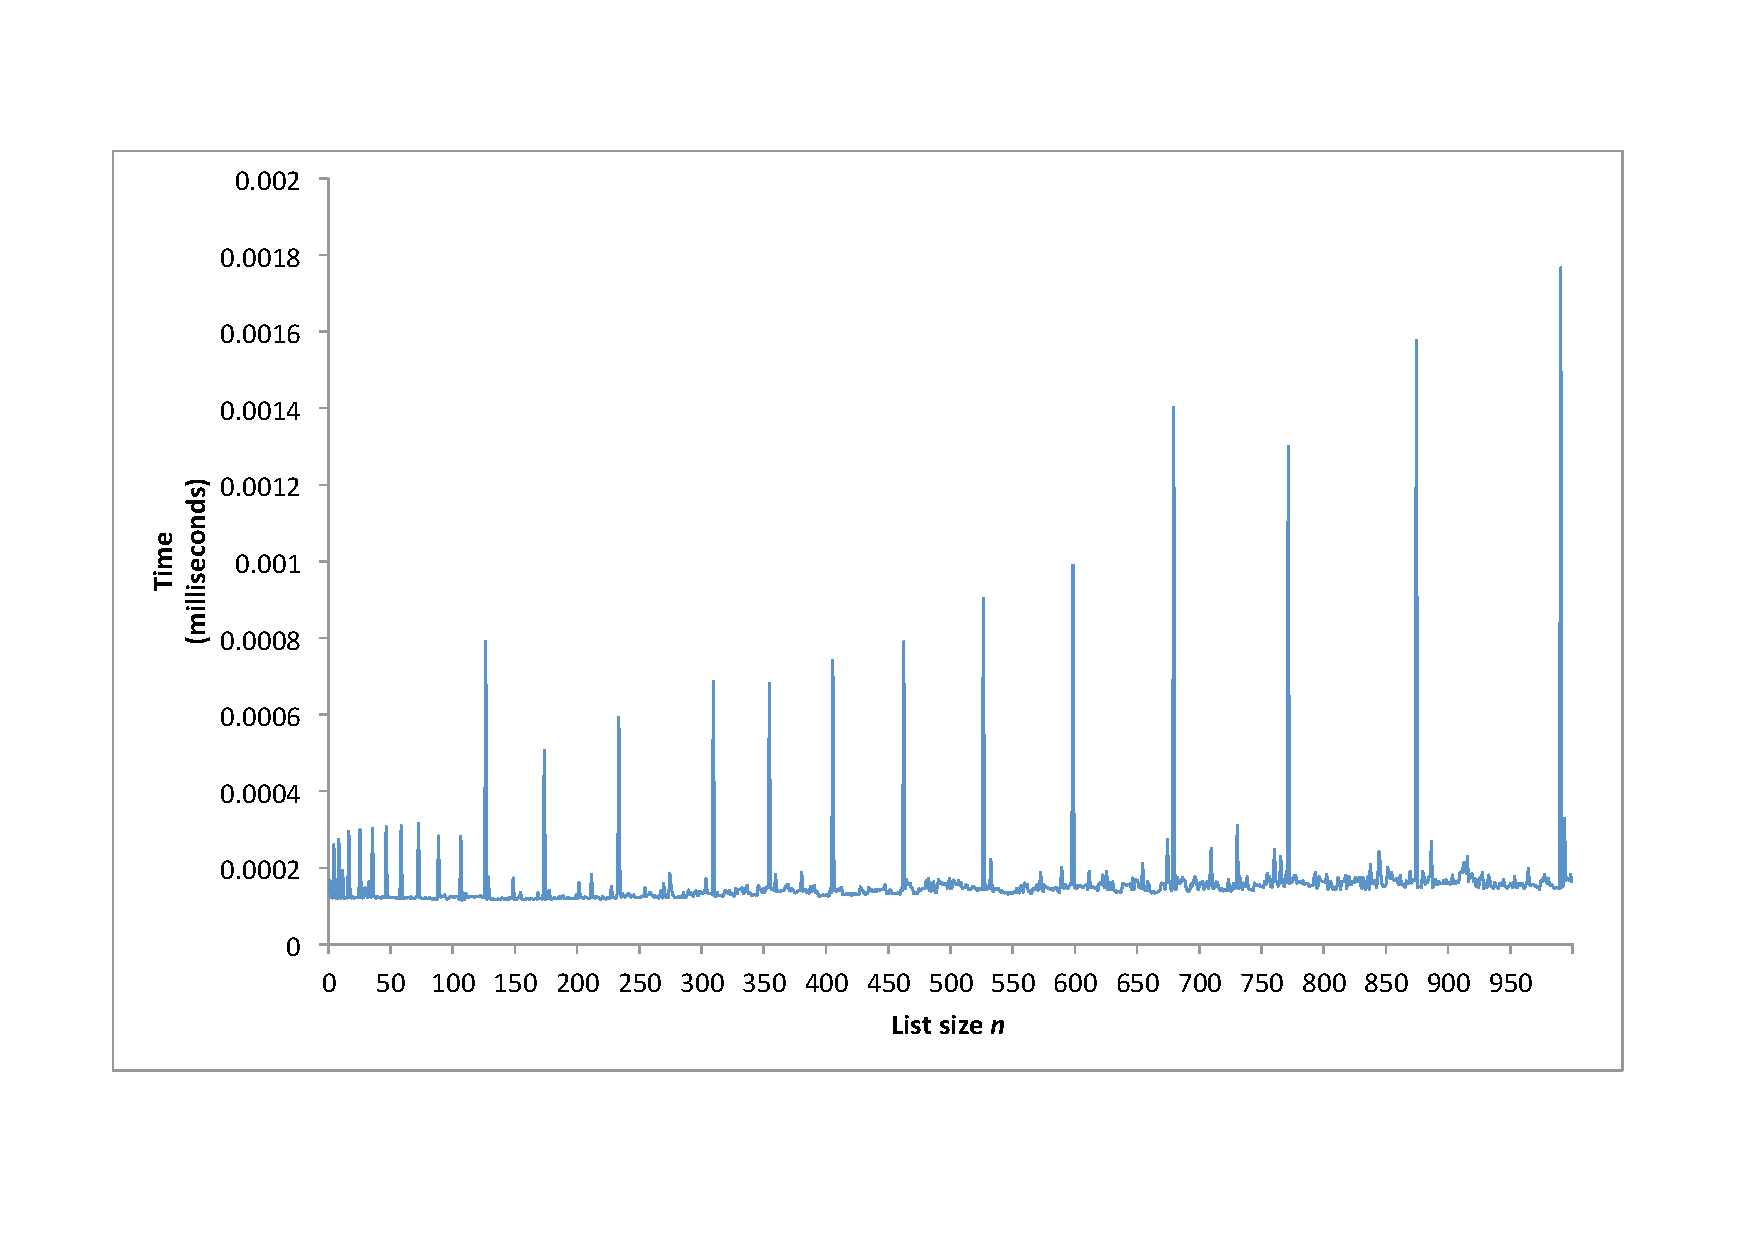
\includegraphics[height=0.9\textheight]{list_append_timing}
	\end{center}
\end{frame}

\begin{frame}{Operations on lists}
	\begin{itemize}
		\pause\item \textbf{Appending} to a list is \textbf{amortised constant time}
			\begin{itemize}
				\pause\item Usually $O(1)$, but can go up to $O(n)$ if the list needs to change size
			\end{itemize}
		\pause\item \textbf{Inserting} anywhere other than the end is \textbf{linear time}
			\begin{itemize}
				\pause\item Can't just insert new bytes into a memory block ---
					need to move all subsequent list elements to make room
			\end{itemize}
		\pause\item Similarly, \textbf{deleting} anything other than the last element is \textbf{linear time}
	\end{itemize}
\end{frame}

\begin{frame}{Tuples}
	\begin{itemize}
		\pause\item Tuples are like lists, but are \textbf{immutable}
			\begin{itemize}
				\pause\item Read-only
				\pause\item Once created, can't be changed
			\end{itemize}
		\pause\item Useful for storing sequences of values where adding, inserting, deleting or
			changing individual values does not make sense
			\begin{itemize}
				\pause\item E.g.\ $xy$ coordinates, RGB colours, ...
			\end{itemize}
		\pause\item Create tuples with \lstinline{()}, just as you create lists with \lstinline{[]}
			\begin{itemize}
				\pause\item Exception: a single element tuple is created as \lstinline{(foo,)}
					because \lstinline{(foo)} would be interpreted as a bracketed expression
			\end{itemize}
		\pause\item Can often omit the parentheses entirely, e.g.\ \lstinline{my_tuple = 1,2,3}
	\end{itemize}
\end{frame}

\begin{frame}[fragile]{Unpacking}
	If \lstinline{foo} is a list or tuple of length 4, the following are equivalent:
	\pause
	\begin{columns}
		\begin{column}{0.48\textwidth}
			\begin{lstlisting}
a, b, c, d = foo
			\end{lstlisting}
		\end{column}
		\pause
		\begin{column}{0.48\textwidth}
			\begin{lstlisting}
a = foo[0]
b = foo[1]
c = foo[2]
d = foo[3]
			\end{lstlisting}
		\end{column}
	\end{columns}
	\begin{itemize}
		\pause\item Unpacking requires the number of elements to match exactly ---
			if \lstinline{foo} has more than 4 elements, the code on the left will give an error
	\end{itemize}
\end{frame}

\begin{frame}[fragile]{One weird trick (Java programmers hate it!)}
	The following are equivalent:
	\pause
	\begin{columns}
		\begin{column}{0.48\textwidth}
			\begin{lstlisting}
a, b = b, a
			\end{lstlisting}
		\end{column}
		\pause
		\begin{column}{0.48\textwidth}
			\begin{lstlisting}
temp = a
a = b
b = temp
			\end{lstlisting}
		\end{column}
	\end{columns}
\end{frame}

\begin{frame}[fragile]{Strings are immutable}
	\begin{itemize}
		\pause\item \textbf{Strings} are immutable in Python
			\begin{itemize}
				\pause\item This is not true of all programming languages
			\end{itemize}
		\pause\item But wait... we change strings all the time, don't we?
	\end{itemize}
	\begin{lstlisting}
my_string = "Hello "
my_string += "world"
	\end{lstlisting}
	\begin{itemize}
		\pause\item This isn't changing the string, it's creating a new one and throwing the old one away!
		\pause\item Hence building a long string by appending can be slow (appending strings is $O(n)$)
	\end{itemize}
\end{frame}

\begin{frame}{Dictionaries}
	\begin{itemize}
		\pause\item Dictionaries are \textbf{associative maps}
		\pause\item A dictionary maps \textbf{keys} to \textbf{values}
			\begin{itemize}
				\pause\item Keys must be immutable (numbers, strings, tuples etc)
				\pause\item Values can be anything (including dictionaries or other containers)
			\end{itemize}
		\pause\item A dictionary is implemented as a \textbf{hash table}
	\end{itemize}		
\end{frame}

\begin{frame}[fragile]{Using dictionaries}
	\pause Create them using \lstinline|{}|:
	\begin{lstlisting}
age = {"Alice": 23, "Bob": 36, "Charlie": 27}
	\end{lstlisting}
	\pause Access values using \lstinline{[]}:
	\begin{lstlisting}
print(age["Alice"]) # prints 23
age["Bob"] = 40     # overwriting an existing item
age["Denise"] = 21  # adding a new item
	\end{lstlisting}
\end{frame}

\begin{frame}[fragile]{Iterating over dictionaries}
	\pause Iterating over a dictionary gives the \textbf{keys}:
	\begin{lstlisting}
for x in age:
    print(x)   # prints Alice, Bob, Charlie
	\end{lstlisting}
	\pause Use \lstinline{items} to get \textbf{key,value} pairs:
	\begin{lstlisting}
for key, value in age.items():
    print(key, "is", age, "years old")
	\end{lstlisting}
\end{frame}

\begin{frame}{Sets}
	\begin{itemize}
		\pause\item Sets are like dictionaries without the values
		\pause\item Sets are \textbf{unordered} collections of \textbf{unique} elements
            \begin{itemize}
                \pause\item Sets \textbf{cannot} contain \textbf{duplicate} elements
                \pause\item Attempting to \lstinline{add} an element already present in the set does nothing
            \end{itemize}
		\pause\item Certain operations on sets scale better on average than the equivalent operations on lists:
	\end{itemize}
	\pause
	\begin{center}
		\begin{tabular}{|c|c|c|}
			\hline
			\textbf{Operation} & \textbf{List} & \textbf{Set} \\\hline
			Add element & Append: $O(1)$ & $O(1)$ \\
			& Insert: $O(n)$ & \\\hline
			Delete element & $O(n)$ & $O(1)$ \\\hline
			Contains element? & $O(n)$ & $O(1)$ \\\hline
		\end{tabular}
	\end{center}
\end{frame}

\begin{frame}[fragile]{Using sets}
    \pause Create them using \lstinline|{}|:
	\begin{lstlisting}
numbers = {1, 4, 9, 16, 25}
	\end{lstlisting}
	\pause Add and remove members with \lstinline{add} and \lstinline{remove} methods
	\begin{lstlisting}
numbers.add(36)
numbers.remove(4)
	\end{lstlisting}
	\pause Test membership with \lstinline{in} operator
	\begin{lstlisting}
if 9 in numbers:
    print("Set contains 9")
	\end{lstlisting}
\end{frame}

\part{2-dimensional arrays}
\frame{\partpage}

\begin{frame}{2-dimensional arrays}
	\pause Common problem: we want to represent a \textbf{2-dimensional array} of values (i.e.\ a grid)
	\pause
	$$
		\begin{matrix}
			v_{0,0} & v_{1,0} & \cdots & v_{w-1,0} \\
			v_{0,1} & v_{1,1} & \cdots & v_{w-1,1} \\
			\vdots  & \vdots  & \ddots & \vdots  \\
			v_{0,h-1} & v_{1,h-1} & \cdots & v_{w-1,h-1}
		\end{matrix}
	$$
\end{frame}

\begin{frame}{Approach 1: flat list}
	\begin{itemize}
		\pause\item For a $w \times h$ array, create a list of size $wh$
		\pause\item The element in column $x$ row $y$ is accessed by \lstinline{list[y * w + x]}
		\pause\item E.g.\ $w=5, h=4$:
		$$
			\begin{matrix}
				0 & 1 & 2 & 3 & 4 \\
				5 & 6 & 7 & 8 & 9 \\
				10 & 11 & 12 & 13 & 14 \\
				15 & 16 & 17 & 18 & 19
			\end{matrix}
		$$
	\end{itemize}
\end{frame}

\begin{frame}{Approach 2: list of lists}
	\begin{itemize}
		\pause\item For a $w \times h$ array, create a list of size $w$, where each element is a list of size $h$
			\begin{itemize}
				\pause\item Each element of the ``outer'' list represents a column of the array
			\end{itemize}
		\pause\item The element in column $x$ row $y$ is accessed by \lstinline{list[x][y]},
			i.e.\ the $y$th element of the $x$th column
	\end{itemize}
\end{frame}

\begin{frame}{Approach 3: dictionary}
	\begin{itemize}
		\pause\item Represent the array as a dictionary whose keys are \lstinline{(x,y)} tuples
		\pause\item The element in column $x$ row $y$ is accessed by \lstinline{list[x, y]}
	\end{itemize}
\end{frame}

\begin{frame}{Approach 4: NumPy array}
	\begin{itemize}
		\pause\item Requires NumPy or SciPy, and can only store numeric types
		\pause\item However, highly optimised for intensive calculations
			(e.g.\ ``tinkering'' with image pixel colours...?)
	\end{itemize}
\end{frame}

\begin{frame}{Which is best?}
	\begin{itemize}
		\pause\item Flat list is reasonably efficient but not very readable
		\pause\item List of lists is a reasonable trade-off between efficiency and readability
		\pause\item Dictionary allows for ``sparse'' arrays (e.g.\ some cells can be missing)
		\pause\item NumPy array is less versatile but faster in some use cases
	\end{itemize}
	\pause There is no single ``best'' approach --- it depends how you use it
\end{frame}

\part{More data structures}
\frame{\partpage}

\begin{frame}{Stacks and queues}
	\begin{columns}
		\pause
		\begin{column}{0.3\textwidth}
			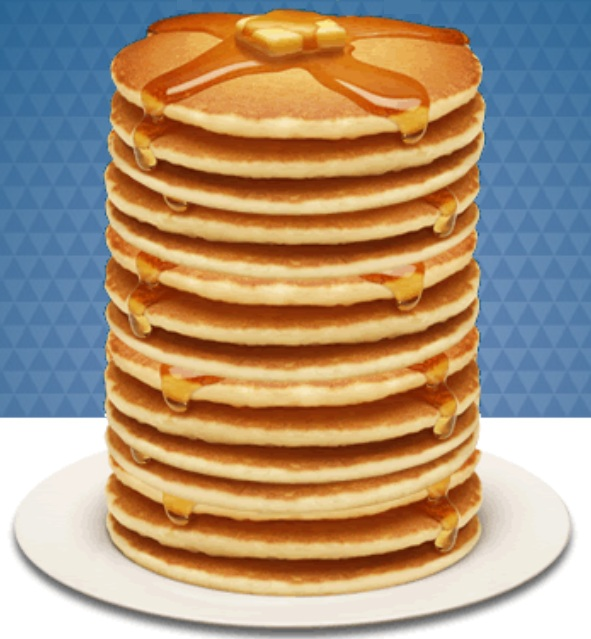
\includegraphics[width=\textwidth]{stack}
		\end{column}
		\begin{column}{0.68\textwidth}
			\begin{itemize}
				\item A \textbf{stack} is a \textbf{last-in first-out (LIFO)} data structure
				\pause\item Items can be \textbf{pushed} to the \textbf{top} of the stack
				\pause\item Items can be \textbf{popped} from the \textbf{top} of the stack
			\end{itemize}
		\end{column}
	\end{columns}
	\begin{columns}
		\pause
		\begin{column}{0.3\textwidth}
			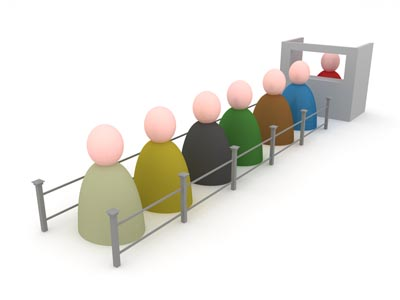
\includegraphics[width=\textwidth]{queue}
		\end{column}
		\begin{column}{0.68\textwidth}
			\begin{itemize}
				\item A \textbf{queue} is a \textbf{first-in first-out (LIFO)} data structure
				\pause\item Items can be \textbf{enqueued} to the \textbf{back} of the queue
				\pause\item Items can be \textbf{dequeued} from the \textbf{front} of the queue
			\end{itemize}
		\end{column}
	\end{columns}
\end{frame}

\begin{frame}{Stacks and queues in Python}
	\begin{itemize}
		\pause\item Stacks can be implemented efficiently as lists
		\pause\item Queues can be implemented as lists, but not efficiently
		\pause\item \lstinline{deque} (from the \lstinline{collections} module) implements an efficient
			\textbf{double-ended queue}
		\pause\item Inserting and removing elements from the start and end of a \lstinline{deque} is $O(1)$
	\end{itemize}
\end{frame}

\begin{frame}{Graphs}
	\begin{columns}
		\pause
		\begin{column}{0.3\textwidth}
			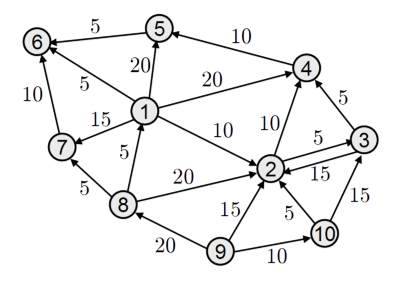
\includegraphics[width=\textwidth]{graph1}
			\par
			\vspace{2ex}
			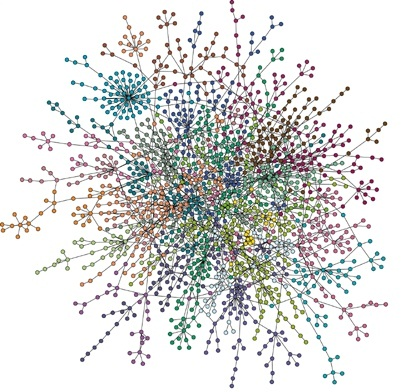
\includegraphics[width=\textwidth]{graph2}
		\end{column}
		\begin{column}{0.68\textwidth}
			\begin{itemize}
				\pause\item A \textbf{graph} is defined by:
					\begin{itemize}
						\pause\item A collection of \textbf{nodes} or \textbf{vertices} (points)
						\pause\item A collection of \textbf{edges} or \textbf{arcs} (undirected lines or directed arrows between points)
					\end{itemize}
				\pause\item Often used to model \textbf{networks} (e.g.\ social networks, transport networks, game levels, finite state automata, ...)
			\end{itemize}
		\end{column}
	\end{columns}
\end{frame}

\begin{frame}{Trees}
	\begin{columns}
		\pause
		\begin{column}{0.3\textwidth}
			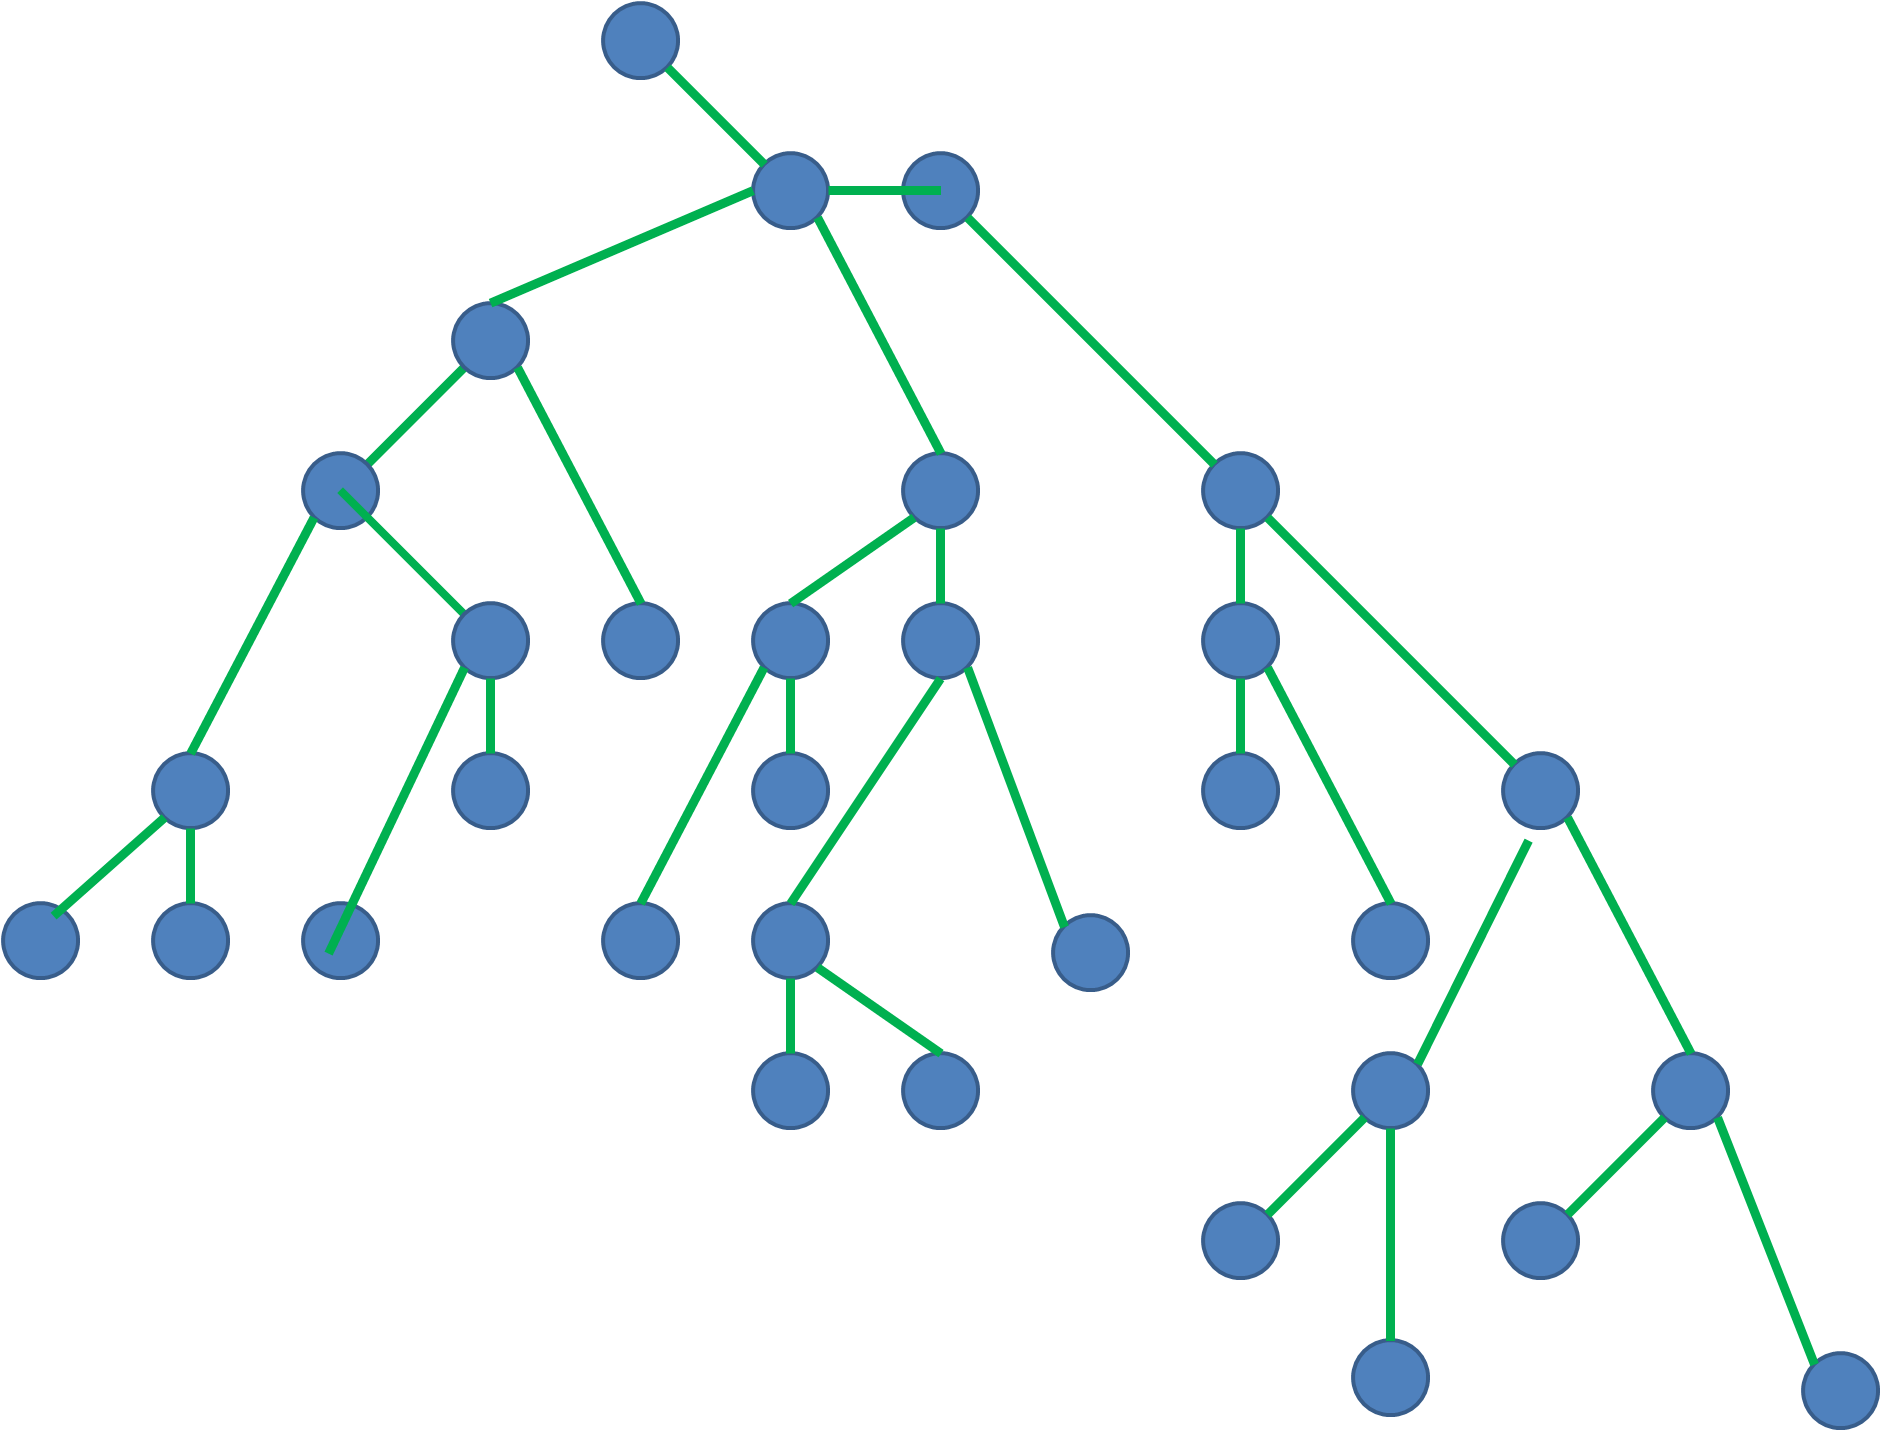
\includegraphics[width=\textwidth]{tree2}
			\par
			\vspace{2ex}
			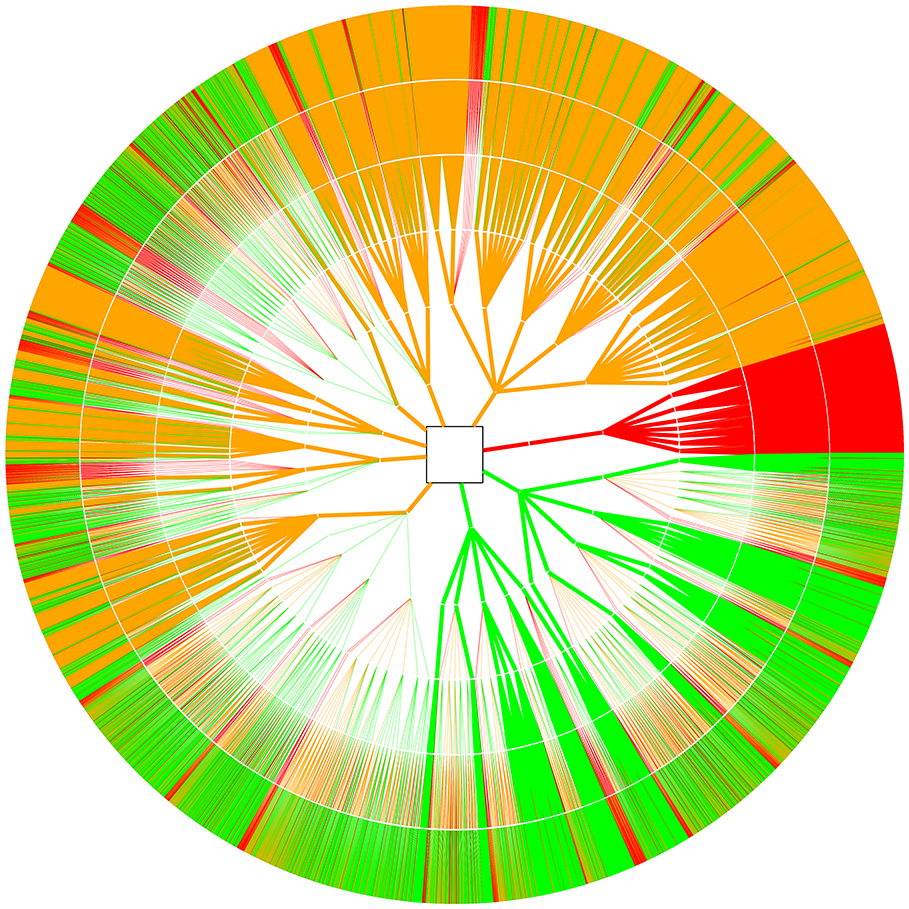
\includegraphics[width=\textwidth]{tree}
		\end{column}
		\begin{column}{0.68\textwidth}
			\begin{itemize}
				\pause\item A \textbf{tree} is a special type of directed graph where:
					\begin{itemize}
						\pause\item One node (the \textbf{root}) has no incoming edges
						\pause\item All other nodes have exactly 1 incoming edge
					\end{itemize}
				\pause\item Edges go from \textbf{parent} to \textbf{child}
					\begin{itemize}
						\pause\item All nodes except the root have exactly one parent
						\pause\item Nodes can have 0, 1 or many children
					\end{itemize}
				\pause\item Used to model \textbf{hierarchies} (e.g.\ file systems, object inheritance, scene graphs, state-action trees, ...)
			\end{itemize}
		\end{column}
	\end{columns}
\end{frame}



\begin{frame}
	\begin{center}
		\textit{``Smart data structures and dumb code works a lot better than the other way around.''}
		
		--- Eric S.\ Raymond
	\end{center}
\end{frame}

\end{document}
